\documentclass[thesis.tex]{subfiles}
\begin{document}

    \chapter*{Introduction}
         \addcontentsline{toc}{chapter}{Introduction}
    \chaptermark{Introduction}
    \markboth{Introduction}{Introduction}
    % The three lines above are to make sure that the headers are right, that the intro gets included in the table of contents, and that it doesn't get numbered 1 so that chapter one is 1.

% Double spacing: if you want to double space, or one and a half
% space, uncomment one of the following lines. You can go back to
% single spacing with the \singlespacing command.
% \onehalfspacing
% \doublespacing

The Milky Way is an entirely unextraordinary galaxy. Its hallmark spiral arms---visible in the night sky as a bright smearing of stars, stretching from horizon to horizon---are shared by about 60\% of galaxies in our universe \citep{apm-bgc}. A bar---a large collection of stars passing through the galactic center, prominent in renderings of the Milky Way (such as Fig. \ref{ssc2008})---is also found around two in three other spiral galaxies. Under the Hubble classification system commonly used to sort and organize galaxies, the Milky Way is classified as an \emph{Sb} type galaxy, along with 40\% of known galaxies (for more information, see \ref{hubble-fork}). These extensive similarities mean that studying the evolution and structure of the Milky Way can provide insights about galactic behavior in general, and that observing other galaxies can reveal the past and future of out own.

\begin{figure}[p]
    \includegraphics[width=\textwidth,height=\textheight,keepaspectratio]{imgs/ssc2008-10a_Sm}
    \caption{This rendering of the Milky Way clearly shows the stellar bar going through the center of the galaxy, and the extensive spiral system. \emph{Image courtesy NASA/JPL}}
    \label{ssc2008}
\end{figure}

\section*{Disks}
The Milky Way has two main disks which hold the vast majority of visible matter in the galaxy and give rise to its spiral structure. The \emph{thin disk} is the more visible of the two, composed mainly of main-sequence stars and clouds of gas and dust \citep{galaxies-in-universe}. Its vertical density scale height---the distance over which its density decreases by a factor of $e$---is about $\SI{350}{\parsec}$---very thin compared to its radius of about $\SI{25}{\kilo\parsec}$. This thinness comes from its young age, since the stars that compose it are less likely to have had their orbits perturbed---especially in the chaotic period about $\SI{9}{\giga\year}$ ago. The thin disk accounts for about 97\% of the galaxy's (normal) mass and holds nearly all galactic dynamism and stellar formation.

The other disk, referred to as the \emph{dark disk} or \emph{thick disk}, is far older and less dynamic \citep{starrfield-thick-disk}. Composed of stars formed $\SI{10}{\giga\year}$ to $\SI{12}{\giga\year}$ ago, it is very faint and hard to detect---all the bright stars burned out long ago, and the only ones left are low-magnitude red dwarfs and K-class stars. These stars' orbits also tend to be less regular, since they've had time to be perturbed and pushed into new orbits, especially during the chaotic initial organization of the Milky Way $\SI{10}{\giga\year}$ ago---resulting in a scale height of about $\SI{1}{\kilo\parsec}$. Because its stars are so steady-burning and the complete lack of gas and dust, the thick disk is very stable and exhibits none of the dynamism seen in the thin disk. It accounts for only about 3\% of the regular matter in the galaxy, with a total mass of about $\SI{1e10}{\solar}$.
Note that the name \emph{dark disk} refers to the low luminosity of the stars within, and has no relation to the dark matter discussed below.

\section*{Metallicity and Age}
The easiest way to determine which disk a star is in is to look at its metallicity (the amount of metal in the star.) This can be measured by looking at the strength of various emission spectra, since elements like iron have very distinct emission lines. These heavy elements are only formed when large stars reach the end of their life, and so their concentration has steadily increased over time as more large stars form and die. Old stars dating back to the formation of the galaxy (like those of the thick disk) tend to have very ``clean'' emission spectra, with very little other than hydrogen and helium, while younger stars have strong magnesium and iron lines.

Metallicity isn't a perfect way to measure the age of a star. Metal concentrations vary widely across both space and time, and two stars forming at the same time may have very different metallicities. However, when looking at a large and statistically representative sample of stars, a high metallicity indicates a younger age \citep[pp. 885]{modern-astrophysics}.

\section*{The Stellar Halo}

The disks extend to about $\SI{25}{\kilo\parsec}$ from the galactic center, and contain practically all the mass within that radius. Past that point, however, stars are distributed far more chaotically. The thin plane disappears, and stellar orbits become more spherically distributed. The composition of individual stars in the halo is similar to those in the thick disk---old, dim, and unchanging. However, the halo is also home to many globular clusters, groups of tens or hundreds of thousands of stars that act like small galaxies in their own right. These clusters continue to create new stars, and most of the light coming from the halo is from globular clusters.

Measurements of stellar velocities have long predicted that the mass of the halo dominates the mass of the galaxy---about 95\% of galactic mass must be in the halo for the observed velocity curves to hold. Since the halo was known not to be made up of gas and dust (otherwise its extinctive properties would be easy to measure), astronomers long though that the halo contained vast numbers of dense, dark bodies, such as lone planets, dim stars, black holes, and neutron stars---referred to as MACHOs, or Massive Astrophysical Compact Halo Object. Gravitational lensing observations disproved this theory, however, when they capped the mass percentage of MACHOs at about 15\% of the mass of the galaxy. The remainder of the mass was some strange material, spherically distributed throughout the universe, that interacts with nothing but gravity.

\section*{Dark Matter}
As that strange material was further studied (as much as it is possible to study something so elusive), more of its properties were discovered. This \emph{dark matter} seems to be made up of WIMPS (Weakly Interacting Massive Particles), which only interact via gravity and the weak force. Being collisionless (since it does not interact with the electromagnetic force), it does not coalesce and form clouds and stars like regular matter, which is how it has maintained its spherical distribution for so long.

This dark matter has a density of
\begin{equation}
    \rho(r) = \frac{\rho_0}{\left(\frac{r}{a}\right)\left(1+\frac{r}{a}\right)^2}
\end{equation}
where $\rho_0$ is the maximum density and $a$ is proportional to the size of the galaxy. This function is referred to as the NFW profile (named after its creators, Navarro, Frank, and White), and is highly accurate for all observed spiral galaxies. For the Milky Way, the simplified equation
\begin{equation}
    \rho(r) = \frac{\rho_0}{1+\left(\frac{r}{1}\right)^2}
\end{equation}
also returns satisfactory results. However, both these equations appear to suffer from a major problem. If we use them to calculate the total mass of the dark matter in a galaxy, integrating from 0 to $\infty$, it appears that a galaxy has an infinite mass, as follows:
\begin{equation}
    \int\limits_{0}^{\infty} \rho(r) 4 \pi r^2 \, \text{d}r = \infty
\end{equation}
Since we know this is not true, there must be a cutoff point where the law no longer holds. As it turns out, in local groups like our own, the dark matter halos are so large that they border one another---providing a natural cutoff point and a solution to our problem \citep[pp. 196]{galaxies-in-universe}.

\section*{Coordinate Systems}

To identify and keep track of objects in the sky, we need to create a coordinate system. A number of natural possibilities spring to mind. The three most useful are detailed below.

\subsection*{Equatorial Coordinates}

An equatorial coordinate has two components---a \emph{right ascension}, and a \emph{declination}. To find this coordinate, find the location on the Earth's surface where the object of interest is directly overhead, in the very middle of the sky. The right ascension is the angle between the nearest point on the equator and the vernal equinox (which is defined to be the point where the equator crosses the ecliptic). The declination is then the angle between the current point and that nearest equatorial point. This coordinate system is very ancient, dating back millennia. Figure \ref{equatorial-coords} shows the process of finding such a coordinate.

\begin{figure}[p]
    \includegraphics{imgs/equat.png}
    \caption{This figure shows the process of finding an equatorial coordinate. CNP and CSP refer to the celestial north and south poles, respectively. R. Ascension refers to the right ascending node, where the Earth's rotational plane crosses its orbital plane.}
    \label{equatorial-coords}
\end{figure}

\subsection*{Galactic Coordinates}

This coordinate system is similar to the equatorial system, but the declination is measured from the galactic plane instead of the equatorial plane. The right ascension is then defined to be the angle between the projection of the body of interest on the galactic plane and the vector between the Sun and galactic center. Figure \ref{galactic-coords} shows this process in more detail. Although harder to calculate from the surface of the earth, this system is more natural when studying bodies traveling close to the Sun. The standard notation and conversions between the two systems are given below:

\begin{tabular}{lll} \toprule
    Measurement & Equatorial Notation & Galactic Notation \\ \midrule
    Right Ascension &  $\delta$       & $b$               \\
    Declination     &  $\alpha$       & $\ell$            \\ \bottomrule
\end{tabular}

\begin{equation}
    \sin b = \sin \delta_{NGP} \sin \delta + \cos \delta_{NGP} \cos \delta \cos (\alpha-\alpha_{NGP})
\end{equation}
\begin{equation}
    \sin \delta = \sin \delta_{NGP} \sin b + \cos \delta_{NGP} \cos b \cos{\ell_{NCP} - \ell}
\end{equation}
Where $\delta_{NGP} = \ang{27;7;41.7}$ and $\ell_{NCP}=\ang{123;55;55.2}$, as determined by the tilt of the earth and its orientation relative to the galactic plane. These equations can also be inverted to find $\ell$ and $\alpha$ \citep[pp. 900]{modern-astrophysics}.

\begin{figure}[p]
    \includegraphics{imgs/galactic}
    \caption{This figure shows the process of finding a galactic coordinate. GNP and GSP refer to the galactic north and south poles, respectively.}
    \label{galactic-coords}
\end{figure}

\subsection*{Cylindrical Coordinates}

The two coordinate systems discussed earlier are well-suited for positional observations from the Earth at a given point in time, but perform poorly over long timeframes. As the sun travels around its orbit, the coordinates of an object change even if it has not moved at all---not an ideal behavior from a reference system. The cylindrical coordinate system, with a reference point at the center of the universe solves these concerns. Unlike the others, it is a three-component coordinate system: $R$ is the radial distance along the plane, increasing outwards; $\theta$ is the angular position, and increases in the direction of rotation; and $z$ is the height above (or below) the plane, increasing towards the north, as shown in figure \ref{cylindrical-coords}. These coordinates also produce a natural (and commonly used) velocity coordinate system, as described below \citep{modern-astrophysics}:
\begin{equation}
    \Pi \equiv \frac{dR}{dt} \hspace{2cm} \Theta \equiv R\frac{d\theta}{dt} \hspace{2cm} Z \equiv \frac{dz}{dt}
\end{equation}

Note that, because the galaxy rotates clockwise when viewed from the north pole, this is a left-handed coordinate system rather than a more-standard right-hand system. Fortunately, we do not need to take any cross-products, so this does not cause any problems.

\begin{figure}[p]
    \includegraphics{imgs/cyl-coords}
    \caption{This figures shows the process of finding a cylindrical coordinate.}
    \label{cylindrical-coords}
\end{figure}

\subsection*{Local Standard of Rest}

Now that we have a definition of the cylindrical velocity coordinates, we can define the Local Standard of Rest (LSR), an important concept in astrophysics. The LSR at a given moment is defined to be the velocity of a body in the sun's position, in a perfectly circular and on-plane orbit---which in practice means the $\Theta$-component of the sun's velocity, with $\Pi$ and $Z$ set to zero.

The velocity of a nearby star relative to the LSR is known as its \emph{peculiar velocity}, and approximates the velocity of that star relative to the sun. Its coordinates are typically designated $(u,v,w)$, where
\begin{align}
    u &= \Pi - \Pi_{LSR} \\
    v &= \Theta - \Theta_{LSR} \\
    w &= Z - Z_{LSR}
\end{align}

The average peculiar velocity for stars in the solar neighborhood is approximately zero, since the universe is mostly axisymmetric. However, individual peculiar velocities vary widely, with young main-sequence stars like the sun having low velocities and old, metal-poor red dwarfs having higher velocities. As discussed earlier, this is due to the additional orbital perturbations experienced by old stars, especially during the chaotic period of formation $\SI{9}{\giga\year}$ ago.
\end{document}
